\documentclass[tikz, varwidth=600pt]{standalone}
\usepackage{amssymb, amsmath,bbm}

\standaloneenv{aaaa}

\begin{document}
	\begin{aaaa}
		\begin{center}	
		\fbox{%
			\begin{minipage}{0.90\linewidth}
				\centering
				\vspace{6pt}
		
		\tikzset{every picture/.style={line width=0.75pt}} %set default line width to 0.75pt        
		
		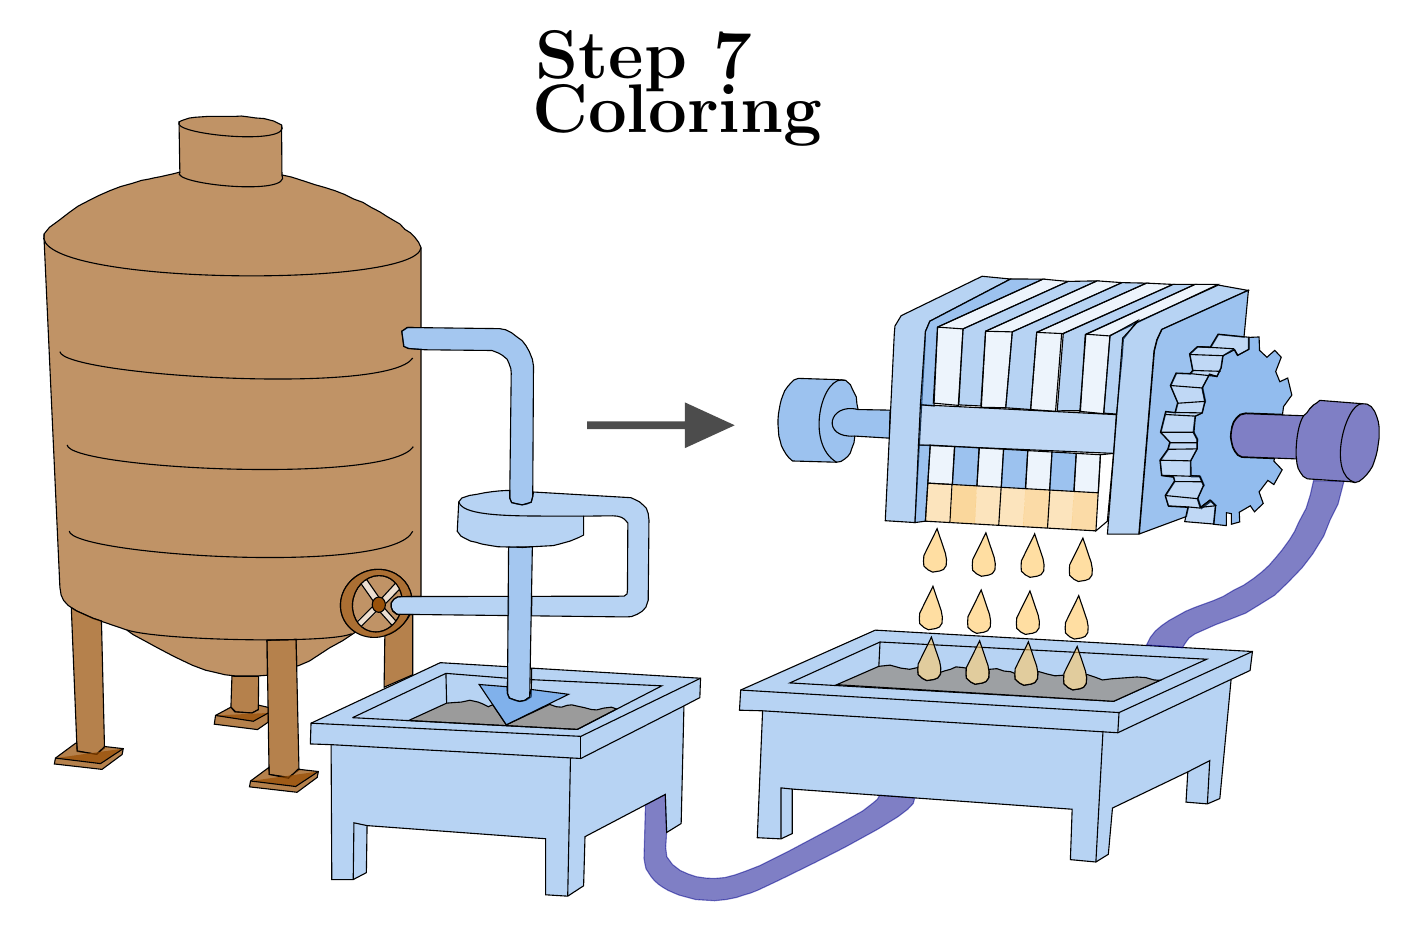
\begin{tikzpicture}[x=0.75pt,y=0.75pt,yscale=-1,xscale=1]
			%uncomment if require: \path (0,464); %set diagram left start at 0, and has height of 464
			
			%Shape: Path Data [id:dp12272833791448257] 
			\draw  [fill={rgb, 255:red, 150; green, 75; blue, 0 }  ,fill opacity=0.6 ] (259.78,268.7) .. controls (265.35,268.7) and (269.76,273) .. (270.76,278.83) -- (268.73,279) -- (266.91,280.09) -- (265.64,281.91) -- (265.64,283.91) -- (266.36,285.73) -- (268.36,287.36) -- (269.77,287.38) .. controls (267.69,292.37) and (263.16,295.9) .. (258.13,295.9) .. controls (251.51,295.9) and (246.51,289.81) .. (246.97,282.3) .. controls (247.43,274.79) and (253.17,268.7) .. (259.78,268.7) -- cycle ;
			%Shape: Path Data [id:dp5328830968083117] 
			\draw  [fill={rgb, 255:red, 150; green, 75; blue, 0 }  ,fill opacity=0.6 ] (212.8,51.6) -- (213,75.7) -- (217.6,76.7) -- (223.2,78.5) -- (228.6,80.3) -- (233.6,81.7) -- (238.6,83.3) -- (243.2,85.1) -- (247.6,87.3) -- (252,88.9) -- (255.6,91.1) -- (260.2,93.5) -- (263.6,95.7) -- (267,97.7) -- (269.8,99.3) -- (272.2,101.9) -- (274.8,103.5) -- (277,105.7) -- (278.8,108.1) -- (280,110.7) -- (280,149.25) -- (273.72,149.18) -- (270.73,151) -- (271.8,158.27) -- (274.24,159.29) -- (280,159.66) -- (280,278.8) -- (275.45,278.81) .. controls (274.31,271.33) and (267.72,265.7) .. (259.4,265.7) .. controls (249.9,265.7) and (241.75,273.04) .. (241.2,282.1) .. controls (240.84,287.94) and (243.74,293.07) .. (248.38,295.98) -- (242.2,300.1) -- (236,303.5) -- (230.8,306.9) -- (226.2,309.9) -- (221,312.1) -- (220.09,312.39) -- (219.8,299.5) -- (205.8,299.9) -- (206.06,316.72) -- (200.8,317.1) -- (191,317.1) -- (185.6,316.5) -- (180.6,315.3) -- (176.2,314.3) -- (169.8,311.9) -- (161,307.7) -- (153,303.5) -- (146.4,299.9) -- (141.2,297.1) -- (138.2,294.9) -- (128.2,291.5) -- (121.8,289.3) -- (114,285.7) -- (110,283.1) -- (107.8,280.7) -- (106.6,278.1) -- (106,274.3) -- (98.4,107.1) -- (98.4,104.1) -- (101,100.9) -- (105.4,97.7) -- (110.6,93.7) -- (114.8,90.7) -- (119.8,88.1) -- (125,85.5) -- (130,83.3) -- (135.2,81.3) -- (141,79.7) -- (145.4,78.3) -- (148.8,77.7) -- (151.4,77.1) -- (154.6,76.5) -- (157.2,75.9) -- (160.8,75.1) -- (163.8,74.3) -- (163.4,50.1) -- (165.2,49.3) -- (168.2,48.3) -- (171.2,47.9) -- (174.2,47.7) -- (177,47.5) -- (190,47.5) -- (193.4,47.3) -- (196.6,47.7) -- (200.29,48.23) -- (204.29,48.51) -- (208.86,49.66) -- (212.8,51.6) -- cycle ;
			%Shape: Polygon [id:ds7417754584469047] 
			\draw  [fill={rgb, 255:red, 150; green, 75; blue, 0 }  ,fill opacity=0.7 ] (219.8,299.5) -- (221.2,362.3) -- (216.2,365.9) -- (206.8,364.5) -- (205.8,299.9) -- cycle ;
			%Shape: Path Data [id:dp7973447942828598] 
			\draw  [fill={rgb, 255:red, 150; green, 75; blue, 0 }  ,fill opacity=0.7 ] (127.5,351.7) -- (123.7,354.84) -- (114.3,353.44) -- (111.5,284.3) -- (111.77,284.31) -- (114,285.7) -- (122.16,289.3) -- (126.03,290.57) -- (127.5,351.7) -- cycle ;
			%Shape: Path Data [id:dp3333829802623004] 
			\draw  [fill={rgb, 255:red, 150; green, 75; blue, 0 }  ,fill opacity=0.7 ] (201.6,333.3) -- (198.6,334.9) -- (190.8,334.5) -- (188.4,332.1) -- (188.9,317.06) -- (190.57,317.3) -- (201.67,317.3) -- (201.77,317.29) -- (201.6,333.3) -- cycle ;
			%Shape: Path Data [id:dp4887073310122587] 
			\draw  [fill={rgb, 255:red, 150; green, 75; blue, 0 }  ,fill opacity=0.7 ] (113.58,349.47) -- (114.18,349.54) -- (114.3,353.17) -- (123.7,354.84) -- (127.5,351.09) -- (127.5,351.06) -- (136.52,352.09) -- (135.99,354.91) -- (126.28,362.09) -- (103.34,359.47) -- (103.87,356.64) -- (113.58,349.47) -- cycle ;
			%Shape: Path Data [id:dp4097819237130982] 
			\draw  [fill={rgb, 255:red, 150; green, 75; blue, 0 }  ,fill opacity=0.7 ] (230.52,363.12) -- (229.99,365.94) -- (220.28,373.12) -- (197.34,370.5) -- (197.87,367.68) -- (206.76,361.1) -- (206.8,364.5) -- (216.2,366.36) -- (220.75,362) -- (230.52,363.12) -- cycle ;
			%Straight Lines [id:da880853432954191] 
			\draw [fill={rgb, 255:red, 150; green, 75; blue, 0 }  ,fill opacity=0.7 ]   (103.87,356.64) -- (125.6,359.3) -- (136.52,352.09) ;
			%Straight Lines [id:da16222466067757924] 
			\draw [fill={rgb, 255:red, 150; green, 75; blue, 0 }  ,fill opacity=0.7 ]   (197.87,367.68) -- (219.6,370.33) -- (230.52,363.12) ;
			%Shape: Polygon [id:ds1925734517222053] 
			\draw  [fill={rgb, 255:red, 150; green, 75; blue, 0 }  ,fill opacity=0.7 ] (188.4,332.1) -- (190.2,334.3) -- (198.6,334.9) -- (201.6,333.3) -- (201.6,331.1) -- (206.3,332.2) -- (206.4,339.3) -- (201.2,342.9) -- (180.4,340.3) -- (181,336.1) -- cycle ;
			%Straight Lines [id:da5107900865309942] 
			\draw [fill={rgb, 255:red, 150; green, 75; blue, 0 }  ,fill opacity=0.7 ]   (181,336.1) -- (199.2,338.9) -- (206.4,334.9) ;
			%Shape: Path Data [id:dp8394684484704809] 
			\draw  [fill={rgb, 255:red, 150; green, 75; blue, 0 }  ,fill opacity=0.7 ] (276,316.5) -- (262.2,322.5) -- (262.57,297.53) .. controls (267.88,295.81) and (272.3,292.12) .. (274.74,287.44) -- (276,287.45) -- (276,316.5) -- cycle ;
			%Curve Lines [id:da20604949679032103] 
			\draw    (110.5,247.3) .. controls (112,258.88) and (266,268.88) .. (276,247.38) ;
			%Curve Lines [id:da8228919822852501] 
			\draw    (109.5,205.8) .. controls (111,217.38) and (264.25,224.88) .. (276.25,206.63) ;
			%Curve Lines [id:da6040030133359005] 
			\draw    (106,160.8) .. controls (107.5,172.38) and (264,182.13) .. (276,163.88) ;
			%Curve Lines [id:da7577823961133989] 
			\draw    (98.4,104.1) .. controls (90.75,128.88) and (277.75,130.63) .. (280,110.7) ;
			%Right Arrow [id:dp2731978489474587] 
			\draw  [draw opacity=0][fill={rgb, 255:red, 0; green, 0; blue, 0 }  ,fill opacity=0.7 ] (360,194.43) -- (407.17,194.43) -- (407.17,185.29) -- (431.14,196.29) -- (407.17,207.29) -- (407.17,198.14) -- (360,198.14) -- cycle ;
			%Shape: Polygon [id:ds08267684333118774] 
			\draw  [fill={rgb, 255:red, 74; green, 144; blue, 226 }  ,fill opacity=0.5 ] (314.18,160.27) -- (317.45,161.55) -- (319.27,162.64) -- (321.45,164.45) -- (322.36,166.45) -- (323.27,169) -- (323.45,171.18) -- (322.73,231.36) -- (323.64,233.55) -- (326.36,234.27) -- (328.73,234.64) -- (330.91,234.27) -- (333.09,233.36) -- (333.82,230.64) -- (334.18,167.73) -- (333.64,164.45) -- (332.18,160.82) -- (330.55,157.91) -- (328.73,155.55) -- (326,153.55) -- (323.64,151.73) -- (320.73,150.27) -- (317.82,149.73) -- (273.27,149.18) -- (270.73,151) -- (271.64,158.27) -- (273.71,159.29) -- (281.86,159.92) -- cycle ;
			%Shape: Polygon [id:ds7453379184627046] 
			\draw  [color={rgb, 255:red, 0; green, 0; blue, 139 }  ,draw opacity=0.5 ][fill={rgb, 255:red, 0; green, 0; blue, 139 }  ,fill opacity=0.5 ] (397.67,374.17) -- (398.33,392.5) -- (397.86,399.79) -- (398.43,404.21) -- (401.14,407.93) -- (404.86,410.79) -- (408.71,412.5) -- (412.57,413.79) -- (417.57,414.5) -- (421.57,414.64) -- (426.43,414.21) -- (431.29,412.93) -- (436.14,411.21) -- (443.14,408.5) -- (457.14,401.5) -- (479.71,389.5) -- (492.86,382.07) -- (497.86,378.21) -- (499.86,376.5) -- (501,374.5) -- (517.86,375.79) -- (517.14,378.5) -- (514.43,381.36) -- (509.71,384.93) -- (500,390.93) -- (484.14,399.64) -- (469.86,406.93) -- (452.71,415.36) -- (445.43,418.79) -- (442.43,420.21) -- (438.86,421.64) -- (435.43,422.64) -- (432,423.79) -- (427,424.79) -- (421.43,425.36) -- (416.71,425.07) -- (412.29,424.79) -- (408,423.64) -- (404.29,422.64) -- (401.57,421.5) -- (399,420.36) -- (396.57,418.93) -- (394.29,417.36) -- (392.43,415.64) -- (390.86,413.79) -- (389.57,411.79) -- (388.43,410.07) -- (387.86,407.5) -- (387.43,404.93) -- (388.14,379.21) -- cycle ;
			%Shape: Path Data [id:dp9154364742101909] 
			\draw  [fill={rgb, 255:red, 74; green, 144; blue, 226 }  ,fill opacity=0.4 ] (328.73,234.64) -- (333.09,233.36) -- (333.82,230.64) -- (334.18,228.45) -- (381.09,231.18) -- (383.09,232.09) -- (385.27,233.18) -- (386.91,234.64) -- (388.55,236.27) -- (389.45,238.82) -- (389.82,241.91) -- (389.45,280.64) -- (388.36,283.91) -- (386.55,285.91) -- (384.18,287.36) -- (381.45,288.45) -- (379.09,288.64) -- (333.24,288.11) -- (333.39,278.71) -- (377.82,278.64) -- (379.27,277.55) -- (379.45,275.55) -- (379.64,243.36) -- (378,241.55) -- (376.55,240.64) -- (374.55,240.09) -- (372.36,239.91) -- (358.36,240.09) -- (358.36,249.18) -- (355.82,250.45) -- (351.82,252.09) -- (347.27,253.36) -- (343.64,254.27) -- (333.64,254.82) -- (324.18,255) -- (317.09,254.82) -- (312.55,254.09) -- (309.45,253.55) -- (306.36,252.64) -- (303.82,252.09) -- (301.27,250.82) -- (299.27,249.73) -- (297.45,247.36) -- (298.18,233.18) -- (299.64,231.36) -- (303.45,230.09) -- (306.91,229.55) -- (310.55,228.82) -- (314.36,228.27) -- (317.82,227.91) -- (320.73,227.73) -- (322.73,227.73) -- (322.73,231.36) -- (323.64,233.55) -- (328.73,234.64) -- cycle (268.36,287.36) -- (266.36,285.73) -- (265.64,283.91) -- (265.64,281.91) -- (266.91,280.09) -- (268.73,279) -- (270.91,278.82) -- (322.18,278.73) -- (322.11,287.98) -- (268.36,287.36) -- cycle (324.36,252.27) -- (324.36,252.27) -- (324.36,252.27) -- (324.36,252.27) -- cycle ;
			%Shape: Polygon [id:ds9288353630060115] 
			\draw  [fill={rgb, 255:red, 74; green, 144; blue, 226 }  ,fill opacity=0.5 ] (322.18,255) -- (325.45,255) -- (328.91,255.18) -- (333.64,254.82) -- (332.36,327.18) -- (330,328.82) -- (327.45,329.36) -- (325.09,328.82) -- (322.55,327.73) -- (321.64,325.55) -- cycle ;
			%Shape: Path Data [id:dp31464679042769417] 
			\draw  [fill={rgb, 255:red, 74; green, 144; blue, 226 }  ,fill opacity=0.4 ] (414.67,318.17) -- (414.33,327.5) -- (406.67,331.5) -- (405.33,388.17) -- (398.33,392.5) -- (397.67,374.17) -- (359,394.5) -- (358.33,418.17) -- (350.67,423.17) -- (340,422.5) -- (340,395.5) -- (254,389.17) -- (253.67,411.83) -- (247.33,415.17) -- (237,415.17) -- (236.67,350.17) -- (226.67,349.83) -- (227,339.83) -- (289.27,310.67) -- (321.74,312.61) -- (321.64,325.55) -- (322.61,327.73) -- (325.32,328.82) -- (327.84,329.36) -- (330.55,328.82) -- (333.07,327.18) -- (333.33,313.3) -- (414.67,318.17) -- cycle ;
			%Straight Lines [id:da5828010059710726] 
			\draw    (236.67,350.17) -- (357,356.83) ;
			%Straight Lines [id:da38129706866191726] 
			\draw    (357,356.83) -- (406.67,331.5) ;
			%Straight Lines [id:da8057563293100857] 
			\draw    (227,339.83) -- (357,346.17) ;
			%Straight Lines [id:da2917197006600606] 
			\draw    (357,356.83) -- (357,346.17) ;
			%Straight Lines [id:da2801000707067103] 
			\draw    (247.33,415.17) -- (247.67,387.83) -- (254,389.17) ;
			%Straight Lines [id:da9031030120619815] 
			\draw    (357,346.17) -- (414.67,318.17) ;
			%Straight Lines [id:da9856983259717322] 
			\draw    (247,337.17) -- (292,315.83) -- (321.67,318.17) ;
			%Straight Lines [id:da1134588763918275] 
			\draw    (292.33,330.17) -- (292,315.83) ;
			%Straight Lines [id:da8171783437343805] 
			\draw    (350.67,423.17) -- (352,356.5) ;
			%Shape: Polygon [id:ds15771101735317528] 
			\draw  [color={rgb, 255:red, 0; green, 0; blue, 0 }  ,draw opacity=1 ][fill={rgb, 255:red, 155; green, 155; blue, 155 }  ,fill opacity=1 ] (292.33,330.17) -- (295.78,329.89) -- (299.33,329.67) -- (303.56,328.78) -- (307.56,329.67) -- (309.78,330.56) -- (312.44,331.89) -- (314.55,330.91) -- (321.09,340.64) -- (342,330.78) -- (345.11,331.89) -- (347.78,332.11) -- (350.44,331.22) -- (352.67,331) -- (355.56,331.67) -- (358.67,332.33) -- (362,333.22) -- (364.67,333.44) -- (368,332.56) -- (371.78,332.11) -- (374.22,333) -- (355.33,342.83) -- (274,338.56) -- cycle ;
			%Straight Lines [id:da5464426925954466] 
			\draw    (332.67,318.83) -- (396,321.83) -- (355.33,342.83) -- (247,337.17) ;
			%Shape: Polygon [id:ds8155174455428071] 
			\draw  [fill={rgb, 255:red, 74; green, 144; blue, 226 }  ,fill opacity=0.5 ] (321.45,322.27) -- (321.64,325.55) -- (322.55,327.73) -- (327.45,329.36) -- (330,328.82) -- (332.36,327.18) -- (332.91,323.55) -- (351.09,325.91) -- (321.09,340.64) -- (308,321.18) -- cycle ;
			%Shape: Polygon [id:ds5918954219271793] 
			\draw  [fill={rgb, 255:red, 74; green, 144; blue, 226 }  ,fill opacity=0.4 ] (680.57,305.29) -- (679.43,314.43) -- (670.29,318.71) -- (664.86,376.14) -- (658.86,378.71) -- (648.57,377.86) -- (649.43,363.29) -- (613.14,380.71) -- (611.14,403) -- (605.14,406.71) -- (592.86,405.57) -- (593.71,381.29) -- (458.86,371.57) -- (458.86,393) -- (453.43,395.57) -- (442,395) -- (444.57,333.86) -- (433.43,333.57) -- (434,323.86) -- (498.86,295) -- cycle ;
			%Straight Lines [id:da5102091705680911] 
			\draw    (453.43,395.57) -- (453.43,371) -- (458.86,371.57) ;
			%Straight Lines [id:da590879865753575] 
			\draw    (670.29,318.71) -- (615.71,344.43) -- (444.57,333.86) ;
			%Straight Lines [id:da5246880159731854] 
			\draw    (608.57,343.57) -- (605.14,406.71) ;
			%Straight Lines [id:da2969360619579031] 
			\draw    (658.86,378.71) -- (660,357.86) -- (649.43,363.29) ;
			%Straight Lines [id:da49175517319243434] 
			\draw    (501.14,300.71) -- (457.71,320.43) -- (613.71,329.29) -- (658.57,309) -- cycle ;
			%Straight Lines [id:da8237636735898951] 
			\draw    (680.57,305.29) -- (616.29,334.71) -- (434,323.86) ;
			%Straight Lines [id:da33512604056768447] 
			\draw    (616.29,334.71) -- (615.71,344.43) ;
			%Straight Lines [id:da41235581014965883] 
			\draw    (501.14,300.71) -- (500.57,312.43) ;
			%Shape: Path Data [id:dp5961768989539743] 
			\draw  [fill={rgb, 255:red, 155; green, 155; blue, 155 }  ,fill opacity=0.9 ] (506,311.86) -- (511.14,313.29) -- (515.43,313.86) -- (519.41,313) -- (519.34,314.02) -- (519.52,316.39) -- (521.52,318.2) -- (523.7,319.3) -- (527.16,318.75) -- (528.98,318.02) -- (530.25,316.2) -- (530.3,315.33) -- (532,314.71) -- (535.14,313.86) -- (537.71,312.71) -- (540.86,313) -- (542.75,313.32) -- (542.59,315.77) -- (542.77,318.14) -- (544.77,319.95) -- (546.95,321.05) -- (550.41,320.5) -- (552.23,319.77) -- (553.5,317.95) -- (553.68,315.05) -- (553.48,313.9) -- (554,313.86) -- (557.43,313.57) -- (560.86,314.71) -- (564,315) -- (566.12,315.88) -- (566.09,316.27) -- (566.27,318.64) -- (568.27,320.45) -- (570.45,321.55) -- (573.91,321) -- (575.73,320.27) -- (577,318.45) -- (577.18,315.55) -- (577.09,315.04) -- (577.71,315) -- (581.71,316.14) -- (585.43,317) -- (589.43,316.71) -- (589.71,316.73) -- (589.59,318.52) -- (589.77,320.89) -- (591.77,322.7) -- (593.95,323.8) -- (597.41,323.25) -- (599.23,322.52) -- (600.5,320.7) -- (600.68,317.8) -- (600.44,316.43) -- (601.14,316.43) -- (604.57,317.57) -- (608.29,319) -- (612.86,318.43) -- (624.86,317.57) -- (629.14,317.86) -- (633.14,319) -- (636.14,319.14) -- (613.71,329.29) -- (480.29,321.29) -- (500.57,312.43) -- (506,311.86) -- cycle ;
			%Shape: Polygon [id:ds2878766972255671] 
			\draw  [fill={rgb, 255:red, 255; green, 200; blue, 100 }  ,fill opacity=0.6 ] (575.64,248.64) -- (579.64,260.45) -- (580.18,263.55) -- (580,266.45) -- (578.73,268.27) -- (576.91,269) -- (573.45,269.55) -- (571.27,268.45) -- (569.27,266.64) -- (569.09,264.27) -- (569.27,261.55) -- cycle ;
			%Shape: Polygon [id:ds7023886502906521] 
			\draw  [fill={rgb, 255:red, 255; green, 200; blue, 100 }  ,fill opacity=0.6 ] (552.14,248.14) -- (556.14,259.95) -- (556.68,263.05) -- (556.5,265.95) -- (555.23,267.77) -- (553.41,268.5) -- (549.95,269.05) -- (547.77,267.95) -- (545.77,266.14) -- (545.59,263.77) -- (545.77,261.05) -- cycle ;
			%Shape: Polygon [id:ds19911018608829723] 
			\draw  [fill={rgb, 255:red, 255; green, 200; blue, 100 }  ,fill opacity=0.6 ] (528.64,246.14) -- (532.64,257.95) -- (533.18,261.05) -- (533,263.95) -- (531.73,265.77) -- (529.91,266.5) -- (526.45,267.05) -- (524.27,265.95) -- (522.27,264.14) -- (522.09,261.77) -- (522.27,259.05) -- cycle ;
			%Shape: Polygon [id:ds18830974271367973] 
			\draw  [fill={rgb, 255:red, 255; green, 200; blue, 100 }  ,fill opacity=0.6 ] (598.89,250.64) -- (602.89,262.45) -- (603.43,265.55) -- (603.25,268.45) -- (601.98,270.27) -- (600.16,271) -- (596.7,271.55) -- (594.52,270.45) -- (592.52,268.64) -- (592.34,266.27) -- (592.52,263.55) -- cycle ;
			%Shape: Polygon [id:ds11681759137882242] 
			\draw  [fill={rgb, 255:red, 255; green, 200; blue, 100 }  ,fill opacity=0.6 ] (573.39,276.14) -- (577.39,287.95) -- (577.93,291.05) -- (577.75,293.95) -- (576.48,295.77) -- (574.66,296.5) -- (571.2,297.05) -- (569.02,295.95) -- (567.02,294.14) -- (566.84,291.77) -- (567.02,289.05) -- cycle ;
			%Shape: Polygon [id:ds4678995406179466] 
			\draw  [fill={rgb, 255:red, 255; green, 200; blue, 100 }  ,fill opacity=0.6 ] (549.89,275.64) -- (553.89,287.45) -- (554.43,290.55) -- (554.25,293.45) -- (552.98,295.27) -- (551.16,296) -- (547.7,296.55) -- (545.52,295.45) -- (543.52,293.64) -- (543.34,291.27) -- (543.52,288.55) -- cycle ;
			%Shape: Polygon [id:ds501418222882922] 
			\draw  [fill={rgb, 255:red, 255; green, 200; blue, 100 }  ,fill opacity=0.6 ] (526.64,273.89) -- (530.64,285.7) -- (531.18,288.8) -- (531,291.7) -- (529.73,293.52) -- (527.91,294.25) -- (524.45,294.8) -- (522.27,293.7) -- (520.27,291.89) -- (520.09,289.52) -- (520.27,286.8) -- cycle ;
			%Shape: Polygon [id:ds3798642860092565] 
			\draw  [fill={rgb, 255:red, 255; green, 200; blue, 100 }  ,fill opacity=0.6 ] (596.89,278.39) -- (600.89,290.2) -- (601.43,293.3) -- (601.25,296.2) -- (599.98,298.02) -- (598.16,298.75) -- (594.7,299.3) -- (592.52,298.2) -- (590.52,296.39) -- (590.34,294.02) -- (590.52,291.3) -- cycle ;
			%Shape: Polygon [id:ds4720079297654729] 
			\draw  [fill={rgb, 255:red, 255; green, 200; blue, 100 }  ,fill opacity=0.6 ] (525.89,298.39) -- (529.89,310.2) -- (530.43,313.3) -- (530.25,316.2) -- (528.98,318.02) -- (527.16,318.75) -- (523.7,319.3) -- (521.52,318.2) -- (519.52,316.39) -- (519.34,314.02) -- (519.52,311.3) -- cycle ;
			%Shape: Polygon [id:ds6201581175683556] 
			\draw  [fill={rgb, 255:red, 255; green, 200; blue, 100 }  ,fill opacity=0.6 ] (549.14,300.14) -- (553.14,311.95) -- (553.68,315.05) -- (553.5,317.95) -- (552.23,319.77) -- (550.41,320.5) -- (546.95,321.05) -- (544.77,319.95) -- (542.77,318.14) -- (542.59,315.77) -- (542.77,313.05) -- cycle ;
			%Shape: Polygon [id:ds14894107305171855] 
			\draw  [fill={rgb, 255:red, 255; green, 200; blue, 100 }  ,fill opacity=0.6 ] (572.64,300.64) -- (576.64,312.45) -- (577.18,315.55) -- (577,318.45) -- (575.73,320.27) -- (573.91,321) -- (570.45,321.55) -- (568.27,320.45) -- (566.27,318.64) -- (566.09,316.27) -- (566.27,313.55) -- cycle ;
			%Shape: Polygon [id:ds2566457772668381] 
			\draw  [fill={rgb, 255:red, 255; green, 200; blue, 100 }  ,fill opacity=0.6 ] (596.14,302.89) -- (600.14,314.7) -- (600.68,317.8) -- (600.5,320.7) -- (599.23,322.52) -- (597.41,323.25) -- (593.95,323.8) -- (591.77,322.7) -- (589.77,320.89) -- (589.59,318.52) -- (589.77,315.8) -- cycle ;
			%Curve Lines [id:da27143946567169397] 
			\draw    (298.18,233.18) .. controls (300.18,241.55) and (334.36,239.73) .. (358.36,240.09) ;
			%Shape: Polygon [id:ds07285450263263815] 
			\draw  [fill={rgb, 255:red, 74; green, 144; blue, 226 }  ,fill opacity=0.4 ] (508.33,148.5) -- (511.33,143.5) -- (550.33,124.5) -- (564,125.83) -- (525.14,146.14) -- (523,151.17) -- (523,154.5) -- (518,243.17) -- (503.67,242.27) -- (508,152.5) -- cycle ;
			%Shape: Polygon [id:ds015478113285572359] 
			\draw  [color={rgb, 255:red, 0; green, 0; blue, 139 }  ,draw opacity=0.5 ][fill={rgb, 255:red, 0; green, 0; blue, 139 }  ,fill opacity=0.5 ] (710,223) -- (724.67,223.22) -- (721.78,234.33) -- (718,241.89) -- (714.89,249.67) -- (709.56,258.33) -- (704.44,265) -- (697.56,272.11) -- (691.33,278.11) -- (684.22,282.56) -- (677.33,286.78) -- (670,289.67) -- (662.89,292.33) -- (656.89,295) -- (652.89,296.78) -- (650,298.78) -- (648.22,301.22) -- (646.89,303.44) -- (629.56,302.11) -- (631.33,298.56) -- (633.78,295.44) -- (636.89,292.78) -- (640.44,290.33) -- (644.44,288.11) -- (648.44,285.89) -- (652.67,284.11) -- (656.89,282.56) -- (661.78,280.78) -- (666.44,278.78) -- (671.33,275.89) -- (676.22,273.44) -- (681.11,270.11) -- (685.33,266.78) -- (688.67,263.67) -- (691.78,260.11) -- (694.89,256.33) -- (698.44,251.44) -- (700.89,247.44) -- (702.89,243) -- (706.44,236.33) -- (708.44,229.89) -- cycle ;
			%Shape: Polygon [id:ds34397075377680164] 
			\draw  [fill={rgb, 255:red, 74; green, 144; blue, 226 }  ,fill opacity=0.35 ] (615,191.17) -- (613.67,209.83) -- (519.67,205.83) -- (520.6,186.4) -- cycle ;
			%Shape: Polygon [id:ds7337850778891342] 
			\draw  [fill={rgb, 255:red, 74; green, 144; blue, 226 }  ,fill opacity=0.55 ] (525.14,146.14) -- (564,125.83) -- (579.71,125.86) -- (528.86,149) -- (527.14,187) -- (520.6,186.4) -- (523,151.17) -- cycle ;
			%Shape: Polygon [id:ds45638448446640123] 
			\draw  [fill={rgb, 255:red, 74; green, 144; blue, 226 }  ,fill opacity=0.1 ] (579.71,125.86) -- (591.71,127) -- (541.14,149.86) -- (538.86,186.71) -- (526.8,185.62) -- (528.86,149) -- cycle ;
			%Shape: Polygon [id:ds6982763563084057] 
			\draw  [fill={rgb, 255:red, 74; green, 144; blue, 226 }  ,fill opacity=0.4 ] (591.71,127) -- (605.71,126.71) -- (552,151) -- (549.71,187) -- (539.09,186.47) -- (541.14,149.86) -- cycle ;
			%Shape: Polygon [id:ds38265936374155995] 
			\draw  [fill={rgb, 255:red, 74; green, 144; blue, 226 }  ,fill opacity=0.1 ] (605.71,126.71) -- (617.71,127.57) -- (564.86,151.29) -- (561.71,187.86) -- (549.94,187.62) -- (552,151) -- cycle ;
			%Shape: Polygon [id:ds267230081172102] 
			\draw  [fill={rgb, 255:red, 74; green, 144; blue, 226 }  ,fill opacity=0.4 ] (617.71,127.57) -- (629.49,127.81) -- (576.63,151.53) -- (573.71,188.71) -- (561.71,187.86) -- (564.86,151.29) -- cycle ;
			%Shape: Polygon [id:ds0828843048914848] 
			\draw  [fill={rgb, 255:red, 74; green, 144; blue, 226 }  ,fill opacity=0.1 ] (629.49,127.81) -- (642.29,128.43) -- (588.63,152.38) -- (585.71,189.57) -- (573.71,188.71) -- (576.63,151.53) -- cycle ;
			%Shape: Polygon [id:ds30477375947092933] 
			\draw  [fill={rgb, 255:red, 74; green, 144; blue, 226 }  ,fill opacity=0.4 ] (642.29,128.43) -- (652.86,128.43) -- (600,152.71) -- (597.71,189.29) -- (586.51,189.33) -- (589.43,152.14) -- cycle ;
			%Shape: Polygon [id:ds5907167240994373] 
			\draw  [fill={rgb, 255:red, 74; green, 144; blue, 226 }  ,fill opacity=0.1 ] (652.86,128.43) -- (664,128.43) -- (612,153) -- (608.86,190.71) -- (597.4,189.59) -- (600.31,152.41) -- cycle ;
			%Shape: Polygon [id:ds08790706233319667] 
			\draw  [fill={rgb, 255:red, 74; green, 144; blue, 226 }  ,fill opacity=0.4 ] (625.26,145.88) -- (618.4,154.74) -- (617.83,163.02) -- (615.11,190.9) -- (608.97,190.45) -- (611.89,153.26) -- cycle ;
			%Shape: Polygon [id:ds8018767046980229] 
			\draw  [fill={rgb, 255:red, 74; green, 144; blue, 226 }  ,fill opacity=0.4 ] (625.27,146.45) -- (664.13,128.74) -- (678.41,131.31) -- (636.79,150.14) -- (634.46,155.14) -- (633.13,160.48) -- (625.84,248.74) -- (610.7,248.74) -- (618.04,154.29) -- cycle ;
			%Shape: Path Data [id:dp08570840209787234] 
			\draw  [fill={rgb, 255:red, 74; green, 144; blue, 226 }  ,fill opacity=0.55 ] (626.07,248.65) -- (633.35,160.39) -- (634.69,155.06) -- (637.02,150.06) -- (678.64,131.23) -- (676.5,153.85) -- (664.23,152.6) -- (660.48,158.85) -- (654.23,158.6) -- (650.48,162.1) -- (651.98,170.1) -- (650.73,171.6) -- (643.98,171.35) -- (641.23,177.35) -- (644.73,185.6) -- (643.48,190.35) -- (638.98,189.85) -- (636.48,199.85) -- (640.98,204.6) -- (639.98,208.1) -- (636.23,213.35) -- (636.98,220.6) -- (642.73,221.35) -- (643.23,223.35) -- (638.73,230.35) -- (640.23,235.35) -- (649.73,235.85) -- (648.77,240.24) -- (626.07,248.65) -- cycle (658.01,184.69) -- (657.97,184.84) -- (656.67,178.56) -- (656.72,178.47) -- (658.01,184.69) -- cycle (652.6,199.86) -- (652.6,199.89) -- (653.82,202.15) -- (654.23,202.91) -- (654.23,203.23) -- (652.6,200.2) -- (652.6,200.17) -- (652.45,199.89) -- (652.48,199.64) -- (652.6,199.86) -- cycle (651.24,220.47) -- (651.24,220.78) -- (655.47,220.78) -- (657.34,225.14) -- (657.27,225.29) -- (655.47,221.09) -- (651.24,221.09) -- (651.24,220.78) -- (651.12,220.78) -- (651.12,220.47) -- (651.24,220.47) -- cycle (655.78,235.8) -- (655.87,235.74) -- (655.98,236.11) -- (660.73,232.56) -- (663.12,234.91) -- (662.89,235) -- (660.73,232.87) -- (655.98,236.43) -- (655.87,236.05) -- (655.78,236.11) -- (654.45,231.89) -- (654.51,231.76) -- (655.78,235.8) -- cycle ;
			%Shape: Polygon [id:ds5376749160477031] 
			\draw  [fill={rgb, 255:red, 74; green, 144; blue, 226 }  ,fill opacity=0.55 ] (523,242.5) -- (518,243.17) -- (519.67,205.83) -- (525.33,205.83) -- cycle ;
			%Shape: Polygon [id:ds8052853295098896] 
			\draw  [fill={rgb, 255:red, 74; green, 144; blue, 226 }  ,fill opacity=0.1 ] (536,224.83) -- (524.17,224.17) -- (525.33,205.83) -- (537,206.5) -- cycle ;
			%Shape: Polygon [id:ds761836711596981] 
			\draw  [fill={rgb, 255:red, 245; green, 166; blue, 35 }  ,fill opacity=0.3 ] (534.83,243.17) -- (523,242.5) -- (524.17,224.17) -- (535.83,224.83) -- cycle ;
			%Shape: Polygon [id:ds3593222666772876] 
			\draw  [draw opacity=0][fill={rgb, 255:red, 245; green, 166; blue, 35 }  ,fill opacity=0.45 ] (546.83,243.83) -- (535,243.17) -- (536.17,224.83) -- (547.83,225.5) -- cycle ;
			%Shape: Polygon [id:ds8110303314943839] 
			\draw  [draw opacity=0][fill={rgb, 255:red, 245; green, 166; blue, 35 }  ,fill opacity=0.3 ] (558.5,244.5) -- (546.67,243.83) -- (547.83,225.5) -- (559.5,226.17) -- cycle ;
			%Shape: Polygon [id:ds35180986982777185] 
			\draw  [draw opacity=0][fill={rgb, 255:red, 245; green, 166; blue, 35 }  ,fill opacity=0.3 ] (570.17,245.17) -- (558.33,244.5) -- (559.5,226.17) -- (571.17,226.83) -- cycle ;
			%Shape: Polygon [id:ds2114874230300936] 
			\draw  [draw opacity=0][fill={rgb, 255:red, 245; green, 166; blue, 35 }  ,fill opacity=0.4 ] (581.83,245.83) -- (570,245.17) -- (571.17,226.83) -- (582.83,227.5) -- cycle ;
			%Shape: Polygon [id:ds4587852821075691] 
			\draw  [draw opacity=0][fill={rgb, 255:red, 245; green, 166; blue, 35 }  ,fill opacity=0.3 ] (593.5,246.5) -- (581.67,245.83) -- (582.83,227.5) -- (594.5,228.17) -- cycle ;
			%Shape: Polygon [id:ds05594196337831592] 
			\draw  [draw opacity=0][fill={rgb, 255:red, 245; green, 166; blue, 35 }  ,fill opacity=0.4 ] (605.17,247.17) -- (593.33,246.5) -- (594.5,228.17) -- (606.17,228.83) -- cycle ;
			%Shape: Polygon [id:ds6515671610064973] 
			\draw   (610.67,242.5) -- (605.17,247.17) -- (607.33,210.5) -- (613.67,209.83) -- cycle ;
			%Shape: Path Data [id:dp7965904694584066] 
			\draw  [fill={rgb, 255:red, 74; green, 144; blue, 226 }  ,fill opacity=0.6 ] (651.99,199.75) -- (652.88,191.97) -- (656.22,190.42) -- (657.55,184.86) -- (656.22,178.42) -- (659.77,171.75) -- (663.33,172.86) -- (665.33,168.64) -- (666.22,162.86) -- (671.55,159.53) -- (673.33,162.64) -- (678.66,159.75) -- (678.66,153.97) -- (683.77,153.75) -- (683.99,160.2) -- (687.55,163.53) -- (691.33,160.2) -- (694.44,163.53) -- (691.77,170.42) -- (693.77,175.31) -- (697.55,173.53) -- (699.55,181.75) -- (695.55,187.31) -- (695.06,191.03) -- (677.27,190.39) -- (674.64,191) -- (672.81,192.65) -- (671.39,194.7) -- (670.58,197.17) -- (670.17,199.64) -- (669.97,201.9) -- (670.38,204.36) -- (670.98,206.83) -- (672,208.89) -- (673.42,210.74) -- (675.45,211.76) -- (691.18,212.37) -- (690.88,213.53) -- (694.88,217.75) -- (690.88,224.86) -- (687.99,222.86) -- (683.77,228.42) -- (685.77,233.97) -- (681.55,237.97) -- (679.55,235.09) -- (674.22,238.2) -- (674.44,242.86) -- (670.44,243.97) -- (670.44,238.86) -- (667.99,238.42) -- (667.99,244.64) -- (661.77,243.97) -- (662.66,235.09) -- (659.99,232.42) -- (655.33,235.97) -- (653.99,231.75) -- (656.88,225.31) -- (654.88,220.64) -- (650.66,220.64) -- (650.66,213.53) -- (653.77,207.75) -- (653.77,203.09) -- (651.99,199.75) -- cycle ;
			%Shape: Polygon [id:ds7505822351576087] 
			\draw  [fill={rgb, 255:red, 74; green, 144; blue, 226 }  ,fill opacity=0.35 ] (640,235.13) -- (638.5,230.13) -- (643,223.13) -- (642.5,221.13) -- (636.75,220.38) -- (636,213.13) -- (639.75,207.88) -- (640.75,204.38) -- (636.25,199.63) -- (638.75,189.63) -- (643.25,190.13) -- (644.5,185.38) -- (641,177.13) -- (643.75,171.13) -- (650.5,171.38) -- (651.75,169.88) -- (650.25,161.88) -- (654,158.38) -- (660.25,158.63) -- (664,152.38) -- (678.89,153.89) -- (678.89,159.67) -- (673.56,162.56) -- (672.03,159.88) -- (666.44,162.78) -- (665.56,168.56) -- (663.56,172.78) -- (660,171.67) -- (656.44,178.33) -- (657.78,184.78) -- (656.44,190.33) -- (653.11,191.89) -- (652.37,199.98) -- (654,203) -- (654,207.67) -- (650.89,213.44) -- (651.01,220.56) -- (655.24,220.87) -- (657.11,225.22) -- (654.22,231.67) -- (655.64,235.83) -- (660.22,232.33) -- (662.89,235) -- (662,243.89) -- (647.94,242.71) -- (649.5,235.63) -- cycle ;
			%Shape: Polygon [id:ds38439168046421257] 
			\draw  [fill={rgb, 255:red, 0; green, 0; blue, 139 }  ,fill opacity=0.5 ] (705.2,191.7) -- (706.8,190.3) -- (708.2,188.3) -- (710,186.5) -- (711.6,185.5) -- (713,184.3) -- (733.4,185.9) -- (735.8,186.1) -- (737.8,187.3) -- (739.4,189.5) -- (740.4,191.9) -- (741.2,194.5) -- (741.6,197.1) -- (741.6,199.9) -- (741.6,202.5) -- (741.2,205.3) -- (740.8,208.1) -- (740.2,210.7) -- (739.4,213.3) -- (738.4,216.1) -- (737,218.3) -- (735.6,220.1) -- (733.8,221.9) -- (732,223.3) -- (730,223.9) -- (728,223.5) -- (707,222.1) -- (705,220.9) -- (703.6,218.9) -- (702.6,217.1) -- (702,214.7) -- (701.8,212.5) -- (675.6,211.5) -- (673.6,210.5) -- (672.2,208.7) -- (671.2,206.7) -- (670.6,204.3) -- (670.2,201.9) -- (670.4,199.7) -- (670.8,197.3) -- (671.6,194.9) -- (673,192.9) -- (674.8,191.3) -- (677.4,190.7) -- cycle ;
			%Curve Lines [id:da9165450468856924] 
			\draw    (701.8,212.5) .. controls (701.4,212.1) and (701.2,198.1) .. (705.2,191.7) ;
			%Curve Lines [id:da32011855107045506] 
			\draw    (730,223.9) .. controls (716.4,220.1) and (725.2,185.9) .. (733.4,185.9) ;
			%Straight Lines [id:da705462592628317] 
			\draw    (654,158.38) -- (671.78,159.44) ;
			%Straight Lines [id:da24851390042758748] 
			\draw    (650.25,162.19) -- (666.44,162.78) ;
			%Straight Lines [id:da6832817622803936] 
			\draw    (651.75,169.88) -- (665.2,170.3) ;
			%Straight Lines [id:da7069846017018656] 
			\draw    (650.5,171.38) -- (663.56,172.78) ;
			%Straight Lines [id:da8262015387340742] 
			\draw    (641,177.13) -- (656.44,178.33) ;
			%Straight Lines [id:da11427724260398764] 
			\draw    (644.5,185.69) -- (657.78,184.78) ;
			%Straight Lines [id:da3804633733679056] 
			\draw    (643.25,190.13) -- (656.44,190.33) ;
			%Straight Lines [id:da013482556897940201] 
			\draw    (638.8,191.1) -- (653.11,191.89) ;
			%Straight Lines [id:da3967935923355912] 
			\draw    (636.25,199.63) -- (652.22,199.67) ;
			%Straight Lines [id:da45350242044030875] 
			\draw    (639.75,207.88) -- (654,207.67) ;
			%Straight Lines [id:da3531338703996215] 
			\draw    (640.75,204.69) -- (654,204.7) ;
			%Straight Lines [id:da5936263755922281] 
			\draw    (636,213.13) -- (650.89,213.44) ;
			%Straight Lines [id:da8089306445168479] 
			\draw    (636.75,220.38) -- (651.01,220.87) ;
			%Straight Lines [id:da7791997567887828] 
			\draw    (643,223.44) -- (656.6,223.5) ;
			%Straight Lines [id:da8373278999890549] 
			\draw    (638.5,230.13) -- (654.22,231.67) ;
			%Straight Lines [id:da41322740253271695] 
			\draw    (649.5,235.63) -- (655.56,236.2) ;
			%Straight Lines [id:da6239180024090931] 
			\draw    (655.64,235.83) -- (662.66,235.09) ;
			%Straight Lines [id:da40314499970334106] 
			\draw    (528.86,149) -- (541.14,149.86) ;
			%Straight Lines [id:da7893445885424433] 
			\draw    (552,151) -- (564.86,151.29) ;
			%Straight Lines [id:da4995999952052206] 
			\draw    (576.63,151.53) -- (589.43,152.14) ;
			%Straight Lines [id:da1239721010060082] 
			\draw    (600.31,152.41) -- (611.89,153.26) ;
			%Straight Lines [id:da4175134327947947] 
			\draw    (559.5,226.17) -- (558.33,244.5) ;
			%Straight Lines [id:da8183956682238073] 
			\draw    (583,227.5) -- (581.83,245.83) ;
			%Straight Lines [id:da3666993653749261] 
			\draw    (605.17,247.17) -- (535,243.17) ;
			%Shape: Polygon [id:ds6214348650844053] 
			\draw  [fill={rgb, 255:red, 74; green, 144; blue, 226 }  ,fill opacity=0.55 ] (547.83,225.5) -- (536,224.83) -- (537.17,206.5) -- (548.83,207.17) -- cycle ;
			%Shape: Polygon [id:ds20990622198625397] 
			\draw  [fill={rgb, 255:red, 74; green, 144; blue, 226 }  ,fill opacity=0.1 ] (559.67,226.17) -- (547.83,225.5) -- (549,207.17) -- (560.67,207.83) -- cycle ;
			%Shape: Polygon [id:ds8154734804747978] 
			\draw  [fill={rgb, 255:red, 74; green, 144; blue, 226 }  ,fill opacity=0.55 ] (571.33,226.83) -- (559.5,226.17) -- (560.67,207.83) -- (572.33,208.5) -- cycle ;
			%Shape: Polygon [id:ds41109082965389987] 
			\draw  [fill={rgb, 255:red, 74; green, 144; blue, 226 }  ,fill opacity=0.1 ] (583,227.5) -- (571.17,226.83) -- (572.33,208.5) -- (584,209.17) -- cycle ;
			%Shape: Polygon [id:ds8188526906218655] 
			\draw  [fill={rgb, 255:red, 74; green, 144; blue, 226 }  ,fill opacity=0.55 ] (594.67,228.17) -- (582.83,227.5) -- (584,209.17) -- (595.67,209.83) -- cycle ;
			%Shape: Polygon [id:ds8405910360909946] 
			\draw  [fill={rgb, 255:red, 74; green, 144; blue, 226 }  ,fill opacity=0.1 ] (606.33,228.83) -- (594.5,228.17) -- (595.67,209.83) -- (607.33,210.5) -- cycle ;
			%Shape: Polygon [id:ds9163820940007248] 
			\draw  [fill={rgb, 255:red, 74; green, 144; blue, 226 }  ,fill opacity=0.55 ] (490.57,188.71) -- (506,189) -- (505.6,202.5) -- (489,201.5) -- (488.6,204.7) -- (487.6,207.3) -- (486.8,209.7) -- (485.6,211.3) -- (484.2,212.5) -- (482.4,213.7) -- (480.2,214.1) -- (459,213.5) -- (457.2,211.9) -- (455.8,210.1) -- (454.6,208.1) -- (453.6,206.1) -- (453,203.7) -- (452.4,201.5) -- (452.2,198.9) -- (452,196.1) -- (452,193.5) -- (452.2,190.9) -- (452.6,188.5) -- (453,186.3) -- (453.6,183.9) -- (454.4,181.7) -- (455.2,179.7) -- (456.6,177.7) -- (458,176.1) -- (459.6,174.5) -- (461.8,173.7) -- (480.4,174.3) -- (482.4,174.5) -- (484.6,174.7) -- (486.86,176.71) -- (488,179.29) -- (489.71,182.71) -- (490,185.86) -- cycle ;
			%Curve Lines [id:da2701996298665116] 
			\draw    (484.6,174.7) .. controls (473.4,170.7) and (464.6,204.9) .. (480.2,214.1) ;
			%Curve Lines [id:da5708323643735634] 
			\draw    (490.57,188.71) .. controls (476.2,185.1) and (472.4,202.7) .. (489,201.5) ;
			%Curve Lines [id:da5424138696944657] 
			\draw    (163.8,74.3) .. controls (158.57,80.14) and (218.57,86.14) .. (213,75.7) ;
			%Curve Lines [id:da5526942432880885] 
			\draw    (163.6,50.2) .. controls (158.37,56.04) and (218.37,62.04) .. (212.8,51.6) ;
			%Curve Lines [id:da45949747022488974] 
			\draw    (138.2,294.9) .. controls (154.57,300.14) and (236.57,301.57) .. (246.57,296.71) ;
			%Shape: Polygon [id:ds06795628559148048] 
			\draw  [draw opacity=0][fill={rgb, 255:red, 255; green, 255; blue, 255 }  ,fill opacity=0.7 ] (267.9,272.14) -- (269.08,273.33) -- (269.7,275) -- (263.04,282.1) -- (262.18,280.35) -- (260.72,279.74) -- cycle ;
			%Straight Lines [id:da3803625989241415] 
			\draw    (267.9,272.14) -- (261.17,279.46) ;
			%Straight Lines [id:da6558943005717724] 
			\draw    (269.57,275.43) -- (263.04,282.1) ;
			%Shape: Polygon [id:ds23860274642018087] 
			\draw  [draw opacity=0][fill={rgb, 255:red, 255; green, 255; blue, 255 }  ,fill opacity=0.7 ] (250.88,272.32) -- (252.29,271.41) -- (254.04,271.14) -- (259.67,279.08) -- (257.78,279.57) -- (256.89,280.88) -- cycle ;
			%Shape: Polygon [id:ds4206776609351418] 
			\draw  [draw opacity=0][fill={rgb, 255:red, 255; green, 255; blue, 255 }  ,fill opacity=0.7 ] (268.18,291.05) -- (267.14,292.02) -- (265.75,292.48) -- (260.3,286.29) -- (261.77,285.63) -- (262.35,284.37) -- cycle ;
			%Straight Lines [id:da9082056842796645] 
			\draw    (259.67,279.08) -- (253.75,270.54) ;
			%Shape: Polygon [id:ds7025657795975655] 
			\draw  [draw opacity=0][fill={rgb, 255:red, 255; green, 255; blue, 255 }  ,fill opacity=0.7 ] (251.1,293.24) -- (250,291.96) -- (249.5,290.26) -- (256.63,283.63) -- (257.36,285.43) -- (258.78,286.14) -- cycle ;
			%Straight Lines [id:da052620785634135525] 
			\draw    (251.1,293.24) -- (258.38,285.96) ;
			%Straight Lines [id:da8548740336791033] 
			\draw    (249.35,290.91) -- (256.63,283.63) ;
			%Straight Lines [id:da6121707255561654] 
			\draw    (262.35,284.37) -- (267.88,290.57) ;
			%Straight Lines [id:da3607862021001629] 
			\draw    (260.3,286.29) -- (265.83,292.49) ;
			%Straight Lines [id:da5294658094388827] 
			\draw    (256.89,280.88) -- (250.88,272.32) ;
			%Shape: Ellipse [id:dp1311729435362683] 
			\draw  [fill={rgb, 255:red, 150; green, 75; blue, 0 }  ,fill opacity=0.9 ] (256.5,282.75) .. controls (256.5,280.72) and (257.92,279.08) .. (259.67,279.08) .. controls (261.42,279.08) and (262.83,280.72) .. (262.83,282.75) .. controls (262.83,284.78) and (261.42,286.42) .. (259.67,286.42) .. controls (257.92,286.42) and (256.5,284.78) .. (256.5,282.75) -- cycle ;
			%Shape: Path Data [id:dp7514044737943205] 
			\draw  [fill={rgb, 255:red, 150; green, 75; blue, 0 }  ,fill opacity=0.8 ] (259.4,265.7) .. controls (267.72,265.7) and (274.31,271.33) .. (275.45,278.81) -- (270.91,278.82) -- (270.76,278.83) .. controls (269.76,273) and (265.35,268.7) .. (259.78,268.7) .. controls (253.17,268.7) and (247.43,274.79) .. (246.97,282.3) .. controls (246.51,289.81) and (251.51,295.9) .. (258.13,295.9) .. controls (263.16,295.9) and (267.69,292.37) .. (269.77,287.38) -- (274.35,287.43) .. controls (271.63,293.87) and (264.94,298.5) .. (257.4,298.5) .. controls (247.9,298.5) and (240.65,291.16) .. (241.2,282.1) .. controls (241.75,273.04) and (249.9,265.7) .. (259.4,265.7) -- cycle (266.36,285.73) -- (268.36,287.36) -- (266.36,285.73) -- (266.16,285.21) -- (266.36,285.73) -- cycle ;
			
			% Text Node
			\draw (332.33,31) node [anchor=north west][inner sep=0.75pt]  [font=\Huge] [align=left] {\textbf{Coloring}};
			% Text Node
			\draw (334,5) node [anchor=north west][inner sep=0.75pt]  [font=\Huge] [align=left] {\textbf{Step 7}};
			
		\end{tikzpicture}
	    \vspace{6pt}
\end{minipage}}
		\end{center}
	\end{aaaa}
\end{document}